\documentclass[12pt,a4paper]{exam}
\usepackage[utf8]{inputenc}
\usepackage[T1]{fontenc}
\usepackage{amsmath}
\usepackage{amsfonts}
%\usepackage{amssymb}
\usepackage{graphicx}
\usepackage{geometry}
\usepackage{enumitem}

\geometry{a4paper, margin=2cm}

\usepackage{cprotect}

\usepackage{xcolor}
\definecolor{maroon}{cmyk}{0, 0.87, 0.68, 0.32}
\definecolor{halfgray}{gray}{0.55}
\definecolor{ipython-frame}{RGB}{207, 207, 207}
\definecolor{ipython-bg}{RGB}{247, 247, 247}
\definecolor{ipython-red}{RGB}{186, 33, 33}
\definecolor{ipython-green}{RGB}{0, 128, 0}
\definecolor{ipython-cyan}{RGB}{64, 128, 128}
\definecolor{ipython-purple}{RGB}{170, 34, 255}
\usepackage{listings}
\lstdefinelanguage{iPython}{
	morekeywords={access,and,del,except,exec,in,is,lambda,not,or,raise},
	morekeywords=[2]{for,print,abs,all,any,basestring,bin,bool,bytearray,callable,chr,classmethod,cmp,compile,complex,delattr,dict,dir,divmod,enumerate,eval,execfile,file,filter,float,format,frozenset,getattr,globals,hasattr,hash,help,hex,id,input,int,isinstance,issubclass,iter,len,list,locals,long,map,max,memoryview,min,next,object,oct,open,ord,pow,property,range,reduce,reload,repr,reversed,round,set,setattr,slice,sorted,staticmethod,str,sum,super,tuple,type,unichr,unicode,vars,xrange,zip,apply,buffer,coerce,intern,elif,else,if,continue,break,while,class,def,return,try,except,import,finally,try,except,from,global,pass, True, False},
	sensitive=true,
	morecomment=[l]\#,%
	morestring=[b]',%
	morestring=[b]",%
	moredelim=**[is][\color{black}]{@@}{@@},
	%%
	%morestring=[s]{'''}{'''},% used for documentation text (mulitiline strings)
	%morestring=[s]{"""}{"""},% added by Philipp Matthias Hahn
	%%
	%morestring=[s]{r'}{'},% `raw' strings
	%morestring=[s]{r"}{"},%
	%morestring=[s]{r'''}{'''},%
	%morestring=[s]{r"""}{"""},%
	%morestring=[s]{u'}{'},% unicode strings
	%morestring=[s]{u"}{"},%
	%morestring=[s]{u'''}{'''},%
	%morestring=[s]{u"""}{"""}%
	%
	% {replace}{replacement}{lenght of replace}
	% *{-}{-}{1} will not replace in comments and so on
	%literate=
	%{\%}{{{\color{ipython-purple}+}}}1,
	%{á}{{\'a}}1 {é}{{\'e}}1 {í}{{\'i}}1 {ó}{{\'o}}1 {ú}{{\'u}}1,
	%{Á}{{\'A}}1 {É}{{\'E}}1 {Í}{{\'I}}1 {Ó}{{\'O}}1 {Ú}{{\'U}}1
	%{à}{{\`a}}1 {è}{{\`e}}1 {ì}{{\`i}}1 {ò}{{\`o}}1 {ù}{{\`u}}1
	%{À}{{\`A}}1 {È}{{\'E}}1 {Ì}{{\`I}}1 {Ò}{{\`O}}1 {Ù}{{\`U}}1
	%{ä}{{\"a}}1 {ë}{{\"e}}1 {ï}{{\"i}}1 {ö}{{\"o}}1 {ü}{{\"u}}1
	%{Ä}{{\"A}}1 {Ë}{{\"E}}1 {Ï}{{\"I}}1 {Ö}{{\"O}}1 {Ü}{{\"U}}1
	%{â}{{\^a}}1 {ê}{{\^e}}1 {î}{{\^i}}1 {ô}{{\^o}}1 {û}{{\^u}}1
	%{Â}{{\^A}}1 {Ê}{{\^E}}1 {Î}{{\^I}}1 {Ô}{{\^O}}1 {Û}{{\^U}}1
	%{œ}{{\oe}}1 {Œ}{{\OE}}1 {æ}{{\ae}}1 {Æ}{{\AE}}1 {ß}{{\ss}}1
	%{ç}{{\c c}}1 {Ç}{{\c C}}1 {ø}{{\o}}1 {å}{{\r a}}1 {Å}{{\r A}}1
	%{€}{{\EUR}}1 {£}{{\pounds}}1
	%
	%{^}{{{\color{ipython_purple}\^{}}}}1
	%{=}{{{\color{ipython_purple}=}}}1
	%%
	%*{-}{{{\color{ipython_purple}-}}}1
	%{*}{{{\color{ipython_purple}$^\ast$}}}1
	%{/}{{{\color{ipython_purple}/}}}1%%
	%{+=}{{{+=}}}1
	%{-=}{{{-=}}}1
	%{*=}{{{$^\ast$=}}}1
	%{/=}{{{/=}}}1,
	%
	identifierstyle=\color{black}\footnotesize\ttfamily,
	commentstyle=\color{ipython-cyan}\footnotesize\itshape\ttfamily,
	stringstyle=\color{ipython-red}\footnotesize\ttfamily,
	keepspaces=true,
	showspaces=false,
	showstringspaces=false,
	rulecolor=\color{ipython-frame},
	frame=single,
	frameround={t}{t}{t}{t},
	%framexleftmargin=6mm,
	%numbers=left,
	%numberstyle=\color{ipython-cyan},
	backgroundcolor=\color{ipython-bg},
	%   extendedchars=true,
	basicstyle=\footnotesize\ttfamily,
	keywordstyle=[2]\color{ipython-green}\bfseries\footnotesize\ttfamily, 
	keywordstyle=\color{ipython-purple}\bfseries\footnotesize\ttfamily
}

\lstdefinelanguage{iOutput} {
	sensitive=true,
	identifierstyle=\color{black}\small\ttfamily,
	stringstyle=\color{ipython-red}\small\ttfamily,
	keepspaces=true,
	showspaces=false,
	showstringspaces=false,
	rulecolor=\color{ipython-frame},
	%frame=single,
	%frameround={t}{t}{t}{t},
	%backgroundcolor=\color{ipython-bg},
	basicstyle=\small\ttfamily,
}

\lstnewenvironment{ipython}[1][]{\lstset{language=iPython,mathescape=true,escapeinside={*@}{@*}}%
}{%
}

\lstnewenvironment{ioutput}[1][]{\lstset{language=iOutput,mathescape=true,escapeinside={*@}{@*}}%
}{%
}

\title{Financial Market Course 22/23\\ Exam}
\author{Prof. Simone Freschi, Prof. Matteo Sani}
\date{$21^{\mathrm{st}}$ March 2023}

\printanswers
%\noprintanswers
\begin{document}
\maketitle

\begin{center}
\fbox{\fbox{\parbox{5.5in}{\centering
Answer the questions in the spaces provided. If you run out of room for an answer, continue on the page back.}}}
\end{center}

\begin{center}
\vspace{5mm}
\makebox[0.75\textwidth]{Student's name:\enspace\hrulefill}
\end{center}

\section*{Questions}
\vspace{.5cm}
\begin{questions}
  \question
  Consider a set of zero-coupon bonds of face value \$ 100, with maturity 6 months, 9 months and 2 years. The prices of the bonds are as below:
\begin{table}[h]
  \begin{center}
    \begin{tabular}{|l|c|c|}
      \hline
      \textbf{Period} & \textbf{Maturity} & \textbf{Price (\$)} \\ \hline
      Months          & 6                 & 99.00               \\ \hline
      Months          & 9                 & 98.50               \\ \hline
      Years           & 2                 & 94.35               \\ \hline
    \end{tabular}
  \end{center}
\end{table}
Determine the implied yield curve including the one year zero-coupon rate.
\fillwithlines{3cm}
\begin{solution}
Considering simple compounding rates $\textbf{ZCB}=\cfrac{FV}{1+r*t}$, from the first bond we get
\begin{equation*}
  r_{6M} = \frac{FV-P}{Pt_y} = \frac{100 - 99}{99\cdot0.5} = 2.0202\% 
\end{equation*}

Similarly for the second and third bonds
\begin{equation*}
  \begin{gathered}
    r_{9M} = \frac{100 - 98.50}{98.50\cdot0.75} = 2.0305\% \\
    r_{2Y} = \frac{100 - 94.35}{94.35\cdot2.0} = 2.9942\%
 \end{gathered}   
\end{equation*}

To determine the one year zero rate we can linearly interpolate between the nine months and two years values
\begin{equation*}
  \begin{gathered}
    r_{2Y} = r_{9M}\cdot w_{9M} + r_{2Y}\cdot w_{2Y},\quad\left(w_{9M}=\frac{t_{1Y}-t_{9M}}{t_{2Y}-t_{9M}};w_{9M}=\frac{t_{2Y}-t_{1Y}}{t_{2Y}-t_{9M}}\right) \\
    r_{2Y} = 0.020305\frac{0.25}{1.25} + 0.29942 \frac{1}{1.25} = 2.4359\%
  \end{gathered}
\end{equation*}
\end{solution}
%%%%%%%%%%%%%%%%%%%%%%%%%%%%%%%%%%%%%%%%%%%%%%%%%%%%%%%%%%%%%%%%%%%%%%%%%%%%%%%%%%%
\question
Consider different bonds with a face value of \$ 100, with the following coupon rates.

\begin{table}[h]
  \begin{center}
    \begin{tabular}{|l|c|c|c|c|}
      \hline
      \textbf{Maturity}    & 6M    & 1Y     & 1.5Y   & 2Y  \\ \hline
      \textbf{Coupon (\%)} & 3     & 3.50   & 4.50   & 6 \\ \hline
      \textbf{Price (\$)}  & 98.53 & 103.39 & 105.90 & 110.74 \\ \hline
    \end{tabular}
    \end{center}
  \end{table}
Each bond has a semi-annual payment schedule. Applying the bootstrap technique determine the implied yield curve.
\fillwithlines{3cm}
\begin{solution}
Considering the first bond we can deduce that
\begin{equation*}
  P_1 = \frac{FV + C_1}{(1+r_{6M})^{\frac{1}{2}}} \implies r_{6M} = \left(\frac{100}{98.53}\right)^{2} -1 = 3.00\%
\end{equation*}

The second bond has an intermediate copoun (at 6M) before expiry so previous formula becomes

\begin{equation*}
  \begin{gathered}
    P_2 =  \frac{C_2}{(1+r_{6M})^{\frac{1}{2}}} + \frac{FV + C_2}{(1+r_{1Y})} = \frac{3.5}{(1+0.03)^{\frac{1}{2}}} + \frac{103.5}{(1+r_{1Y})} = 3.4486 + \frac{103.5}{(1+r_{1Y})}\\
    r_{1Y} = \left(\frac{103.5}{103.39-3.4486}\right)-1 = 3.56\%
  \end{gathered}
\end{equation*}

Analogously for the third bond

\begin{equation*}
  \begin{gathered}
    P_3 =  \frac{C_3}{(1+r_{6M})^{\frac{1}{2}}} + \frac{C_3}{(1+r_{1Y})} +  \frac{FV+C_3}{(1+r_{1.5Y})^{\frac{2}{3}}} \\
    r_{1.5Y} = \left(\frac{104.5}{105.9-8.7793}\right)^{\frac{2}{3}}-1 = 5.00\%
  \end{gathered}
\end{equation*}

A different programmatical approach relies on the usage of root finding algorithms on the bond pricing equation to determine the unknown rate:
\begin{ipython}
from scipy.optimize import brentq

rate = [0.03, 0.0356, 0.05]
def price(r, F, C, P):
    return C/(1+rate[0])**0.5 + C/(1+rate[1]) + C/(1+rate[2])**1.5 \\
        + (F+C)/(1+r)**2 - P

r = brentq(price, 0, 0.2, args=(100, 100*0.06, 110.74)
print ("{:.3f}".format(r))
\end{ipython}
\begin{ioutput}
0.065
\end{ioutput}
\end{solution}

%%%%%%%%%%%%%%%%%%%%%%%%%%%%%%%%%%%%%%%%%%%%%%%%%%%%%%%%%%%%%
\question
Under the assumption of the Markowitz \emph{Modern Portfolio Theory} (MPT) the asset allocation can be determined by either minimizing the portfolio variance or maximizing the portfolio expected return. Are the two procedure leading to the \textbf{same} portfolio, i.e. the weights are going to be the same in the two cases ? (explain if and when this is the case).
\fillwithlines{3cm}
\begin{solution}
The resulting portfolios will have the maximum expected return and the lowest risk respectively hence the asset allocation won't be necessarily the same. In order to get the same weights it is necessary to add additional condition on either on the target return or on the target risk.
\end{solution}

%%%%%%%%%%%%%%%%%%%%%%%%%%%%%%%%%%%%%%%%%%%%%%%%%%%%%%%%%%%%%
\question
Consider a portfolio whose efficient frontier is described by the following curve and assume that a risk-free investment yields $r_f = 10\%$.
\begin{center}
  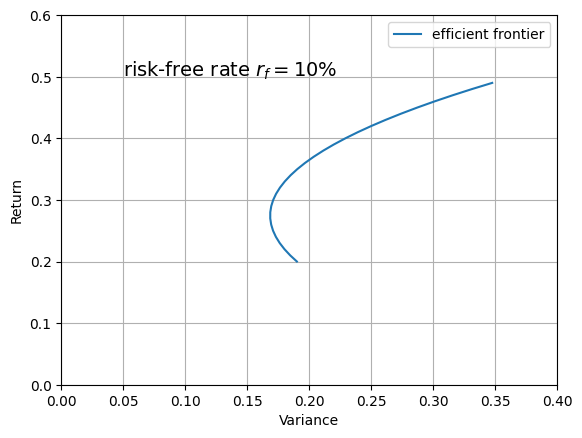
\includegraphics[width=0.7\linewidth]{efficient_frontier}
\end{center}
Using the plot determine the numerical value of the Sharpe ratio corresponding to the asset allocation of the portfolio maximizing it.
\fillwithlines{3cm}
\begin{solution}
In the Variance-Return plane the Sharpe portfolio can be identified by the tangent point between the efficient frontier and the CAL (the line passing through $(0.0, r_f)$. From the given plot this point lies approximately at $(0.2, 0.37)$ so
\begin{equation*}
  SR = \frac{r_P - r_f}{\sigma_P} = \frac{0.37-0.1}{0.2} \approx 1.35
\end{equation*}
\end{solution}

%%%%%%%%%%%%%%%%%%%%%%%%%%%%%%%%%%%%%%%%
\question
Company A finances itself by issuing a 5 year zero-coupon bond. Knowing that the bond is currently sold at \$ 83.75 and that similar riskless ZCB value is \$ 86.07, determine Company A default probability (assume the recovery rate to be 40\%).
\fillwithlines{3cm}
\begin{solution}
The bond price is related to the default probability $\delta$ through the following formula
\begin{equation*}
  P_{bond} = (1-\delta)P_{rf} + \delta P_{rf} R \implies \delta = \frac{P_{bond}-P_{rf}}{P_{rf}(R-1)}
\end{equation*}

Applying previous result to the problem gives a default probability of
\begin{equation*}
  \delta = \frac{83.75-86.07}{86.07\cdot(0.4-1)} \approx 4.5\% 
\end{equation*}
\end{solution}

%%%%%%%%%%%%%%%%%%%%%%%%%%%%%%%%%%%%%%%%%
\question
Let us consider at date $t$, a bond with $FV = \$ 100$, an annual coupon rate of 7\% and time-to-maturity 3 years (T - t = 3 years).
Let also imagine that at date $t$ the market price of the bond at \$ 112.
Suppose that, at date $t$, ZCBs with face value equal to \$ 1, are traded with residual maturity of 1, 2 and 3 years.
Finally assume that the market prices are $B_{1Y} = 0.98$, $B_{2Y} = 0.94$ and $B_{3Y} = 0.90$.
Is there an arbitrage opportunity? Why?
\fillwithlines{3cm}
\begin{solution}
The no-arbitrage price of the bond is
\begin{equation*}
  P = (0.07\cdot100)\cdot 0.98 + (0.07\cdot100)\cdot 0.94 + (100 + 0.07\cdot100)\cdot 0.90 = 109.74
\end{equation*}

This price is smaller than the quoted price hence buying an appropriate number of $B_{1Y}$, $B_{2Y}$ and $B_{3Y}$ and selling the coupon bearing bond it is possible to make a positive net profit.

In particular buying 7 $B_{1Y}$, 7 $B_{2Y}$ and 107 $B_{3Y}$ the profit is \$ 2.26.
\end{solution}

%%%%%%%%%%%%%%%%%%%%%%%%%%%%%%%%%%%%%%%%%%%%
\question
Write a \texttt{python} function that returns the interest rate given the discount factor $D(0, t)$.
\fillwithlines{3cm}
\begin{solution}
  \begin{ipython}
import numpy as np

def r(d, t):
    return np.log(d)/t
  \end{ipython}
\end{solution}
%%%%%%%%%%%%%%%%%%%%%%%%%%%%%%%%%%%%%%%%%%%
\question
Write a \texttt{python} function that compute a coupon-bearing bond price given: notional, coupon, risk-free rate, time-to-maturity, and tenor.
\textbf{Note:} for simplicity consider a flat risk-free rate.
\fillwithlines{3cm}
\begin{solution}
  \begin{ipython}
def bond_price(N, C, r, ttm, tau):
    price = 0
    for t in range(1, ttm+1):
        price += N*tau*C/(1+r)**t
    price += N/(1+r)**t
    return price    
    \end{ipython}
\end{solution}
%%%%%%%%%%%%%%%%%%%%%%%%%%%%%%%%%%%%%%%%%%%
\question
Given the following \texttt{python} expression

\begin{ipython}
a = 36 / 4 * (3 +  2) * 4 + 2

print (a)
\end{ipython}

What is the resulting value stored in variable $a$

\begin{checkboxes}
\choice 182.0
\choice 117
\choice 42
\end{checkboxes}
\begin{solution}
  The solution is 182.0 because of the operator precedence that is preserved in a \texttt{python} expression.
\end{solution}
%%%%%%%%%%%%%%%%%%%%%%%%%%%%%%%%%%%%%%%%%%%
\question
What is the output of the following \texttt{python} code

\begin{ipython}
mylist = [1,2,3,4,5]*3
\end{ipython}
\fillwithlines{3cm}
\begin{solution}
Contrary to one may expect the output will be
\begin{ioutput}
[1,2,3,4,5,1,2,3,4,5,1,2,3,4,5]
\end{ioutput}
and NOT
\begin{ioutput}
[3,6,9,12,15]
\end{ioutput}
\end{solution}
%%%%%%%%%%%%%%%%%%%%%%%%%%%%%%%%%%%%%%%%%%%
\question
What is the output of the following \texttt{python} code

\begin{ipython}
for x in range(0.5, 5.5, 0.5):
    print(x)
\end{ipython}
\fillwithlines{3cm}
\begin{solution}
The program will resul in a
\begin{ioutput}
TypeError: 'float' object cannot be interpreted as an integer
\end{ioutput}
since the built-in function \texttt{range} accepts only integers arguments. To use floats must move to \texttt{np.arange} which is more general.
\end{solution}
%%%%%%%%%%%%%%%%%%%%%%%%%%%%%%%%%%%%%%%%%%%
\question
What is the output of the following \texttt{python} code

\begin{ipython}
def func(n):
    return 1 if n <= 1 else n * factorial(n - 1)

print (func(4))
\end{ipython}
\fillwithlines{3cm}
\begin{solution}
This is a particular implementatio of the factorial function using recursion. Recursion is a particular technique which consists in
calling a function from within itself. It is quite a powerful tool but it must be handled with care since it may easily result in
undesired behaviour. So the answer is
\begin{ioutput}
24
\end{ioutput}
\end{solution}
%%%%%%%%%%%%%%%%%%%%%%%%%%%%%%%%%%%%%%%%%%%%
\question
What is the output of the following code?

\begin{ipython}
var1 = 1
var2 = 2
var3 = "3"

print(var1 + var2 + var3)
\end{ipython}
\fillwithlines{3cm}
\begin{solution}
The result is an error, cannot mix integers and strings in an operation
\begin{ioutput}
TypeError: unsupported operand type(s) for +: 'int' and 'str'
\end{ioutput}
\end{solution}
%%%%%%%%%%%%%%%%%%%%%%%%%%%%%%%%%%%%%%%%%%
\question
What is the difference between a \texttt{for} and a \texttt{while} loop ?
\fillwithlines{3cm}
\begin{solution}
The for loop is used when we know the number of iterations, that is, how many times a statement must be executed. That is why, when we initialize the for loop, we must define the ending point.

A while loop is used when the number of iterations is unknown. It is used when we need to end the loop on a condition other than the number of repetitions. It is not necessary to know the condition ahead of time in this case. That is why we can use a boolean expression in the loop's initialization.
\end{solution}
%%%%%%%%%%%%%%%%%%%%%%%%%%%%%%%%%%%%%%%%%%
\question
Which is a valid variable name in \texttt{python} 

\begin{checkboxes}
\choice \texttt{1\_data}
\choice \texttt{old-data}
\choice \texttt{prince\_in\_\$}
\choice \texttt{\_output}
\end{checkboxes}
\begin{solution}
The only valid variable name is \texttt{\_output} since: cannot start with a number, cannot contain operators (e.g. \texttt{-}), and special characters like \texttt{\$}.
\end{solution}
%%%%%%%%%%%%%%%%%%%%%%%%%%%%%%%%%%%%%%%%%%
\question
Assuming the variable \texttt{myvar} is initialized with 0, which of the following is an \emph{incorrect} assignment statement
in \texttt{python} ?

\begin{checkboxes}
\choice myvar = myvar + 6.99
\choice myvar + 6.99 = myvar
\choice myvar += 6.99
\choice None of the above
\end{checkboxes}
\begin{solution}
The second answer is the correct one.
\end{solution}
%%%%%%%%%%%%%%%%%%%%%%%%%%%%%%%%%%%%%%%%%%
\question
Suppose \texttt{my\_list} is \texttt{[3, 6, 12, 24, 5, 10, 15, 20]}.
Which of the following statements returns the following list \texttt{[6, 24, 10, 20]} ?

\begin{checkboxes}
\choice \texttt{print (my\_list[1:8])}
\choice \texttt{print (my\_list[::2])}
\choice \texttt{print (my\_list[1::2])}
\choice \texttt{print (my\_list[-1:-7:-2])}
\end{checkboxes}
\begin{solution}
Choice 3 is the correct one, since the operator params are \texttt{[start:end:step]}
\end{solution}
%%%%%%%%%%%%%%%%%%%%%%%%%%%%%%%%%%%%%%%%%%
\question
What value is returned by a function that doesn't have a return statement ?

\begin{checkboxes}
\choice None
\choice 0
\choice 1
\choice False
\end{checkboxes}
\begin{solution}
\texttt{None}
\end{solution}
%%%%%%%%%%%%%%%%%%%%%%%%%%%%%%%%%%%%%%%%%%
\question
What is the output of the following code ?

\begin{ipython}
d = {"apple":10, "pear":4, "orange":3}

print (d["peach"])
\end{ipython}
\makeemptybox{3cm}
\begin{solution}
\texttt{KeyError: 'peach'}
\end{solution}
%%%%%%%%%%%%%%%%%%%%%%%%%%%%%%%%%%%%%%%%%%
\question
What should we put instead of the \texttt{?} to make the following boolean expression \texttt{True} ?
\begin{ipython}
True and False or ?
\end{ipython}
\fillwithlines{3cm}
\begin{solution}
You need \texttt{?=True} since the boolean operators have the same precedence so the expression is evaluated from left to right.
Hence
\begin{equation*}
  \begin{gathered}
    \underbrace{\texttt{True and False}}_{\texttt{False}}\texttt{ or ?} = \texttt{True} \\
    \texttt{False or ?} = \texttt{True} \implies \texttt{?} = \texttt{True} \\
    \end{gathered}
\end{equation*}
\end{solution}

%%%%%%%%%%%%%%%%%%%%%%%%%%%%%%%%%%%%%%%%%%

\end{questions}
\end{document}
